\section{Auditor Extension} \label{sec:auditor}
Until now we have not verified whether a certificate chain is logged as promised
by any issued SCT.  Our base design can be extended to follow-up on inclusion
statuses rather than opting for cross-logging.  In terms of
the number of necessary changes, this extension is more significant when
compared to Section~\ref{sec:log}.  However, it does not require any log
modifications, and it entails additional ecosystem value by providing a
well-audited view of the CT landscape which is captured by the Tor consensus.
It is possible to detect internal inconsistency attacks within the Tor
network and omission attacks.  Trust in some logs is also shifted towards CT
auditors.

\subsection{Design Sketch}
\subsection{Security Sketch}

%
% Tor consensus
% - At minimum, same logs as Tor Browser's CT policy
% - Need STH+MMD in ct-log-info, not log's public key
% - Need auditors' public keys pinned
% - Need watchdog timeout
% - Need auditor timeout
%

%
% Phase 1---Tor Browser
% - No changes
%

%
% Phase 2---Storage
% - Small differences
%   --> discard unrecognized SCTs based on ct-log-info entries (change step 2).
%   Note entirely sure if this makes that much of a difference tho with regards
%   to flushing, as the attacker can stuff their submissions large anyway...
%   But it makes the next steps easy, as we only have recognized SCTs around.
%   --> sample one SCT, note down the outcome (add step 3.5)
%   --> compute audit after timestamp based on MMD (change step 4)

%
% Phase 3---Auditing
% - Major differences
%   --> establish connection to a random watchdog (add step 1.75)
%   --> step 3 needs a complete rewrite from (b) and forward
%
% Step 3
% b) continue if SFO.audit_after > STH.timestamp
% c) Submit SFO to watchdog
% d) Use ct-query-timeout and STH.treesize to set a timer and challenge the log
% to prove inclusion.
% - On valid proof: send ACK to watchdog, cache SFO, discard SFO from buffer
% - On any other outcome: discard SFO and break the loop
%
% Behavior of watchdog:
% - Listen for submissions on a dedicated endpoint
% - If a submitted SFO is not ACKed within the watchdog timeout
%   --> submit it to an announced auditor.
%   --> resubmit later on if auditor(s) unavailable; not entirely sure which
%   details we should go with here for the resubmission(s)
%

%
% Extra-info document
% - Need flushing statistics
%

%
% MISC notes
% - Network-wide flush, detectable but hard to attribute
% - Requires new reliable auditor software
% - Bit more bandwidth due to watchdog.  The overhead, when compared to log a
% log extension, is sending an SCT hash and receiving a proof (2-3KiB).
%


\begin{figure*}
    \centering
    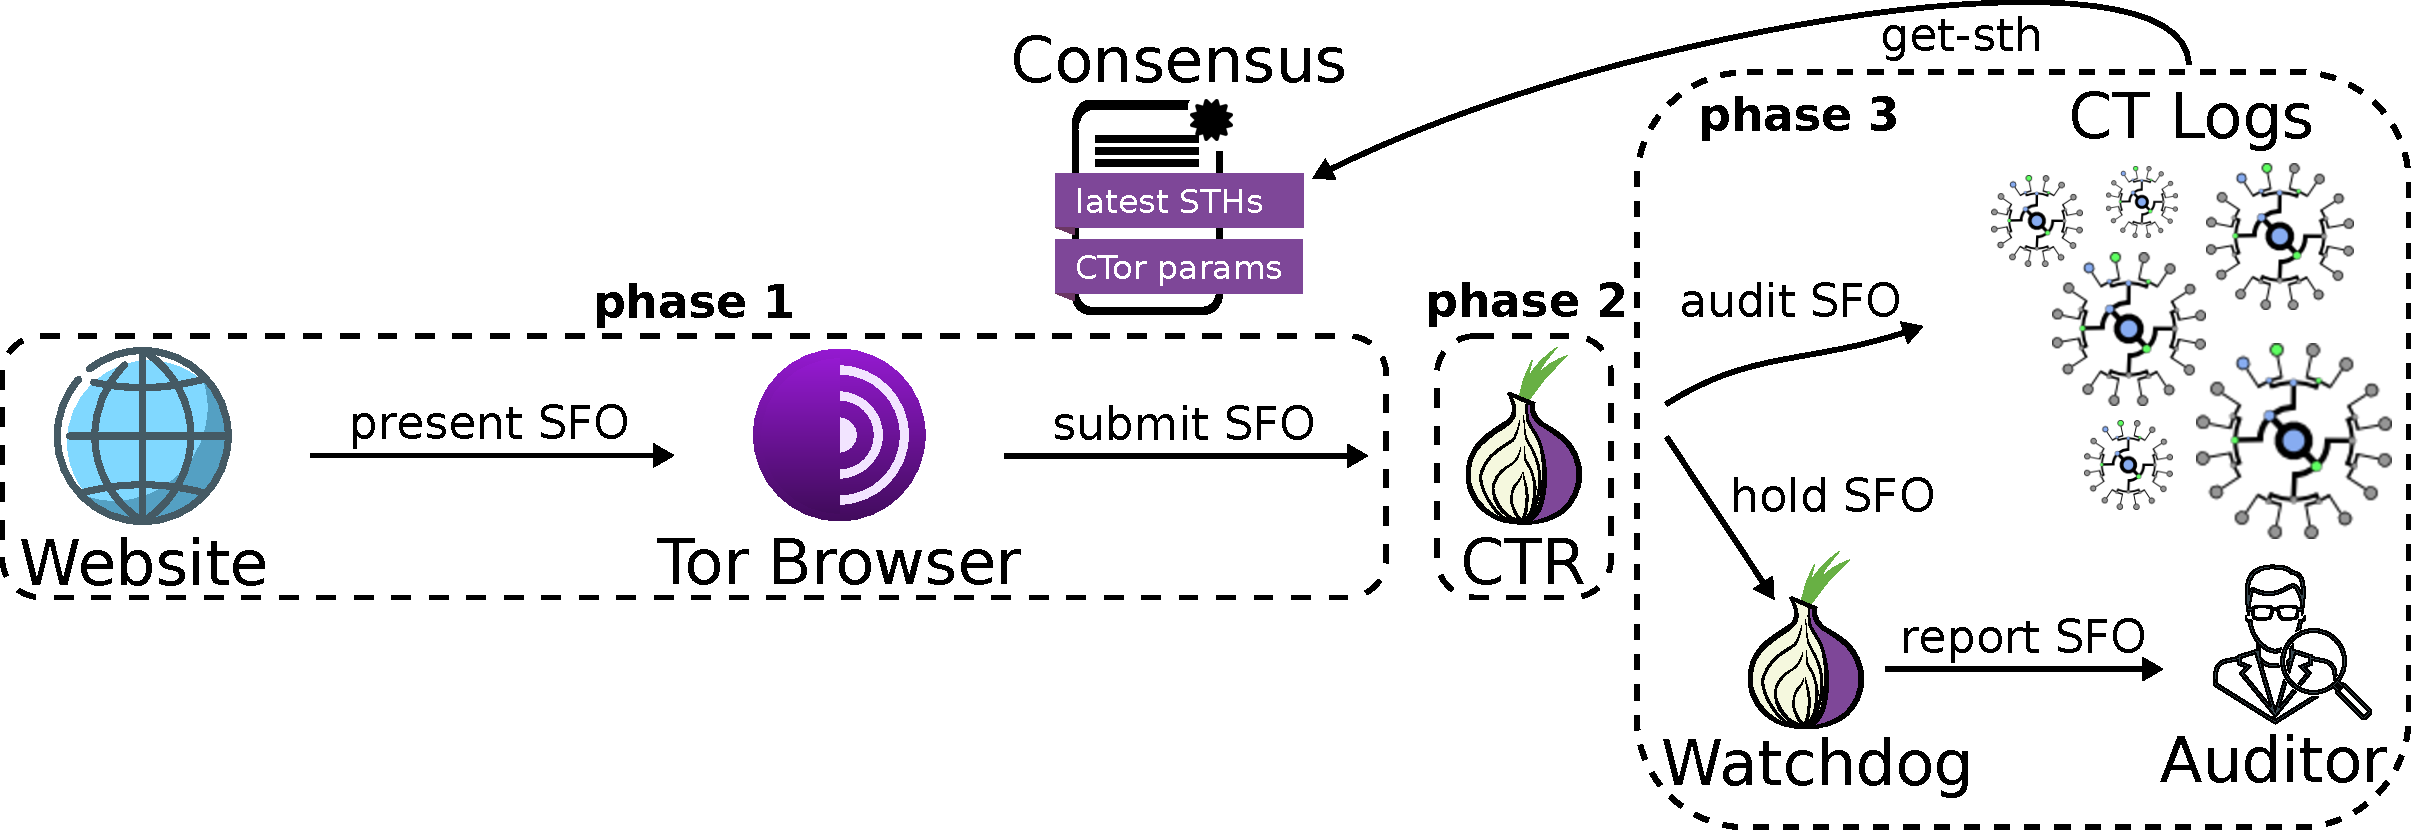
\includegraphics[width=0.85\textwidth]{img/design-auditor}
    \caption{todo}
    \label{fig:design-auditor}
\end{figure*}
